
\section{Fundamentação Teórica}

O envelhecimento populacional tem provocado um aumento significativo na incidência de doenças neurodegenerativas, especialmente o Alzheimer e a Demência Frontotemporal (DFT). Segundo a Organização Mundial da Saúde, mais de 55 milhões de pessoas vivem com demência no mundo, sendo a maior parte delas em países de baixa e média renda \cite{who2021}.

\subsection{Alzheimer e Demência Frontotemporal}

O Alzheimer é caracterizado por deterioração progressiva da memória, linguagem e função cognitiva \cite{alzheimer-association}, enquanto a DFT afeta principalmente o comportamento, a personalidade e a linguagem, sendo de início mais precoce. A Figura~\ref{fig:comparacao} apresenta uma comparação entre as principais características dessas condições.

\begin{figure}[h]
\centering
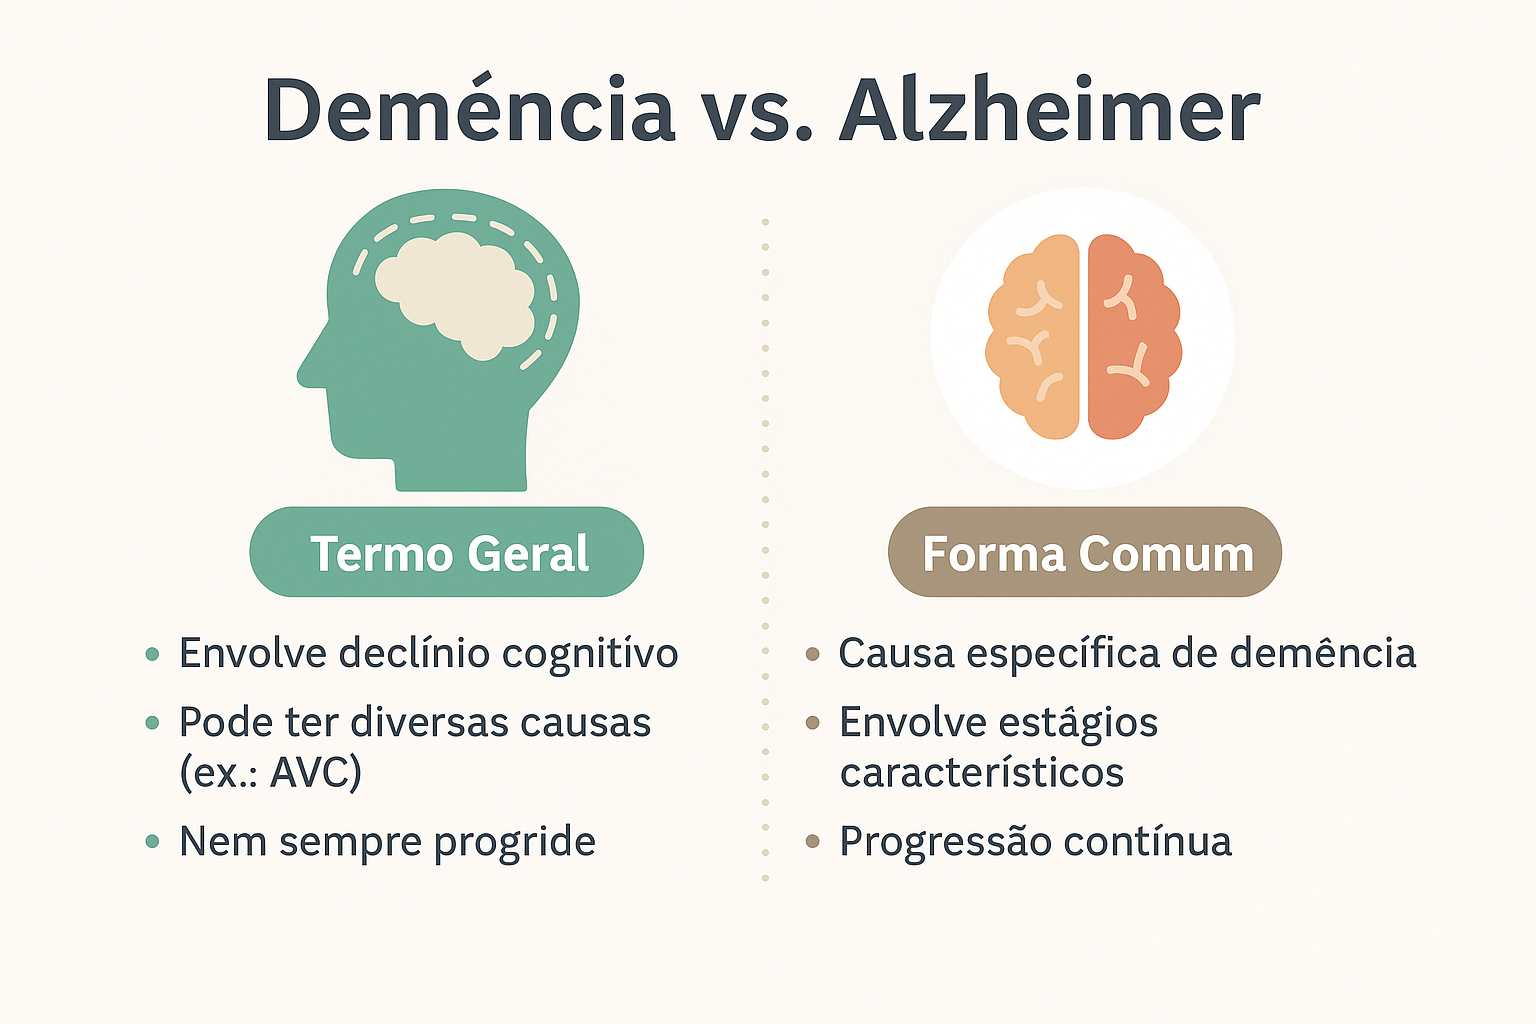
\includegraphics[width=0.7\textwidth]{exemplo-demencia-vs-alzheimer.png}
\caption{Comparação entre Alzheimer e Demência Frontotemporal. Fonte: Adaptado de \cite{alzheimer-association}.}
\label{fig:comparacao}
\end{figure}

\subsection{Tecnologias Assistivas com Inteligência Artificial}

As tecnologias assistivas vêm sendo aprimoradas com a integração da inteligência artificial (IA), permitindo desde assistentes virtuais até ferramentas de reconhecimento de emoções. Soluções que utilizam IA generativa, como os modelos Transformers \cite{huggingface2023}, possibilitam a criação de agentes conversacionais personalizados para públicos vulneráveis.

\begin{table}[h]
\centering
\caption{Tecnologias aplicáveis ao suporte cognitivo de idosos}
\label{tab:tecnologias}
\begin{tabular}{|p{4cm}|p{7cm}|}
\hline
\textbf{Tecnologia} & \textbf{Aplicação no projeto Memória Viva} \\ \hline
Reconhecimento de voz (Web Speech API) & Captura de perguntas feitas pelo idoso de forma natural \\ \hline
Reconhecimento facial (face-api.js) & Identificação biométrica segura do paciente \\ \hline
IA generativa (Hugging Face) & Respostas personalizadas com base em histórico de memórias \\ \hline
Banco de dados Supabase & Armazenamento de perfis, memórias e interações \\ \hline
\end{tabular}
\end{table}

A incorporação dessas ferramentas permite que o sistema interaja com o idoso de maneira empática, auxiliando não apenas na orientação diária, mas também na preservação de vínculos afetivos e da identidade pessoal, aspectos frequentemente comprometidos nessas enfermidades \cite{assistiva2024}.
